\chapter{GPU and OpenCL}
\label{chap:arch}
``OpenCL (Open Computing Language) is an open royalty-free standard
for general purpose parallel programming across CPUs, GPUs and other
processors, giving software developers portable and efficient access
to the power of these heterogeneous processing platforms''
\cite{cl-spec}

\section{Introduction}

In the 1980s, graphics processing units (GPU) began as coprocessors
assisting the central processing units (CPU) with graphics related
computations like drawing lines, arcs, rectangles. GPUs evolved from
these early graphics-oriented instruction sets, specializing in
manipulating and altering images. The parallel nature of graphics
processing, doing the same computations on multiple elements,
eventually led to GPUs with a highly parallel architecture.

General purpose computing on graphics processing units (GPGPU) are
GPUs that are able to perform calculations for applications typically
only run by central processing units (CPU). GPUs are high-performance
many-core processors specialized for compute-intensive and highly
parallel computations, capable of very high throughput. They are
designed with data processing in mind, compared to a CPU which is more
specialized in caching and flow control, as illustrated in figure
\ref{fig:cpu-vs-gpu}. The GPUs parallel throughput architecture
emphasizes executing many concurrent threads slowly, unlike the CPU
that aims to execute a single thread very quickly.

Earlier GPGPUs required the use of graphics programming APIs like
OpenGL and Cg, which limited the general purpose programming
capability tremendously. But in 2007, Nvidia released CUDA, a
proprietary GPGPU framework, which supports parallel programming on a
GPU in C, closely followed by OpenCL in 2008.

\begin{figure}
  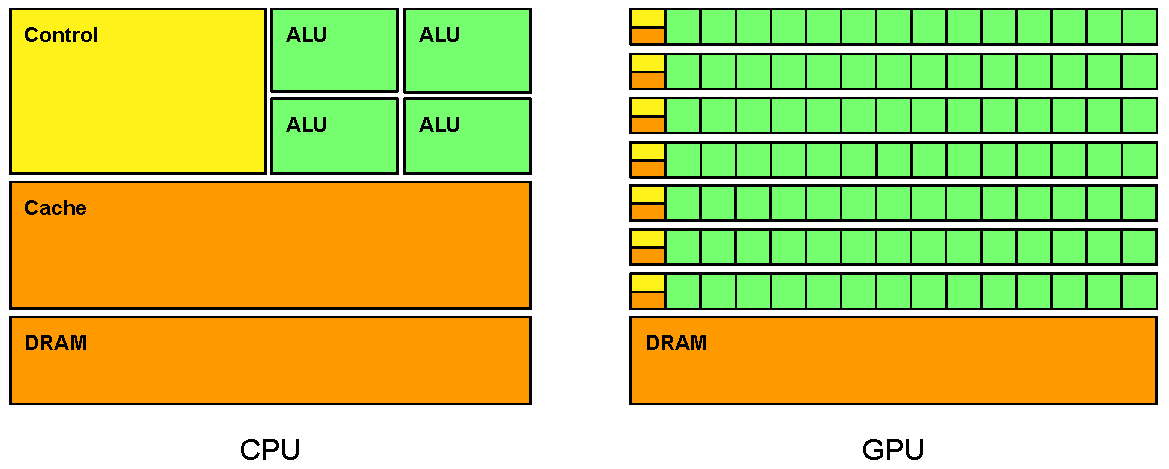
\includegraphics[width=0.8\textwidth]{images/cpu-vs-gpu.pdf}
  \caption{GPUs devote more transistors to data processing than CPUs}
  \label{fig:cpu-vs-gpu}
\end{figure}


\section{OpenCL}

OpenCL was initially proposed by Apple in 2008 and refined in
collaboration with teams from AMD, IBM, Intel and Nvidia. The initial
proposal was submitted to the Khronos Group\cite{cl-spec}, who later
that year released the first OpenCL specification.

The specification is designed as a framework for programming a
heterogeneous collection of CPUs, GPUs and other computing devices
organized into platforms. OpenCL provides low-level hardware
abstraction and an API that supports the underlying hardware to allow
for portable and efficient code. Being a specification and not a
technology in itself, OpenCL needs to be implemented by vendors who
wish to be able to run OpenCL applications and brand themselves OpenCL
compliant. The largest vendors of parallel computing devices have
implementations for OpenCL 1.1 on most operating systems, including
IBM's Power7\cite{ibm-opencl}, most of Nvidias
GPUs\cite{nvidia-opencl}, most of AMDs CPUs and GPUs \cite{amd-opencl}
and Intels CPUs \cite{intel-opencl}.

As frameworks, OpenCL is very similar to Nvidias Compute Unified
Device Architecture (CUDA), but very unlike other parallel computing
frameworks like Hadoop\cite{hadoop} and OpenMP\cite{openmp}. CUDA
currently only works on Nvidia GPUs, while OpenCL currently supports a
number of GPUs, CPUs, DSPs and a number of other accelerator devices.
Additionally, OpenCL also supports task-parallelism, which contrasts
data-parallelism in that the different threads works on different
data or even entirely separate problems.

\subsection{The OpenCL Specification}

The core ideas behind OpenCL are described in a hierarchy of four
models\cite{cl-spec}:

\begin{enumerate}
  \item Platform model
  \item Execution model
  \item Memory model
  \item Programming model
\end{enumerate}

This section contains a condensed summary of the OpenCL specification
without going to in-depth, just to give a basic understanding of how
it works.

% \vspace{10mm}
% \textbf{Platform model}:
\subsubsection{Platform model}

``An OpenCL Platform is defined as a host connected to one or more
OpenCL devices. An OpenCL device is divided into one or more compute
units which are further divided into one or more processing elements.
Computations on a device occur within the processing elements.''
\cite{cl-spec}

\begin{figure}
  \centering
  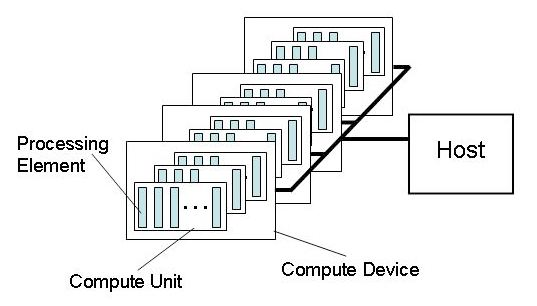
\includegraphics[width=0.8\textwidth]{images/platform-model.png}
  \caption{Platform model, one host plus one or more compute devices,
    each with one or more compute units, each with one or more
    processing elements}
  \label{platform-model-figure}
\end{figure}

An OpenCL device is a collection of compute units. Any processor that
conforms to the OpenCL specification can be a device, ranging from
GPUs, CPUs to DSPs and Cell Broadband Engine processors. A compute
unit is an abstraction for the number or cores the processor has.

A typical home computer usually contains 2 OpenCL compatible devices;
a multi-core CPU and a GPU. Most vendors of consumer CPUs and GPUs
(Intel, AMD, ATI and Nvidia) have OpenCL implementations for their
respective devices available for Linux, OSX and Windows.

The machine used to benchmark the implementation in this thesis, an
Intel i7 CPU and an Nvidia GTX 460, forms 2 platforms. Both Intel and
Nvidia provides an OpenCL implementation for the CPU and the GPU
respectively, and can both be used as OpenCL devices. The host for
both platforms is the CPU device.

\subsubsection{Execution model}

``Execution of an OpenCL program occurs in two parts: kernels that
execute on one or more OpenCL devices and a host program that executes
on the host. The host program defines the context for the kernels and
manages their execution.'' \cite{cl-spec}

When a kernel is submitted for execution, the host defines an index
space. Each point in this index space will be executed by an instance
of the kernel. The index space is called an N-Dimensional Range, or
NDRange, where N can be 1, 2 or 3, and is defined as an N dimensional
integer array. The length of each dimension defines how many
work-items will be launched. The NDRange is often mapped to the
dimensions of either the input or output data.

Work-items can be identified by its coordinates in the index space,
called a global ID. Work-items are further organized into work-groups,
which provides a more coarse grained decomposition of the NDRange.
Work-groups are also uniquely identifiable with a work-group ID.
Work-items in a work-group are assigned a unique ID local to that
work-group. Work-items within a work-group execute concurrently on the
processing elements of a single compute unit.

Figure \ref{execution-model-figure} shows a 2-dimensional NDRange of
$G_x \times G_y$ work-items, organized into $W_x \times W_y$
work-groups, each having $S_x \times S_y$ work-items. A work-item can
be identified multiple ways; by its global ID, by a combination of the
work-group size and ID and the work-items local ID.

\begin{figure}[h]
  \centering
  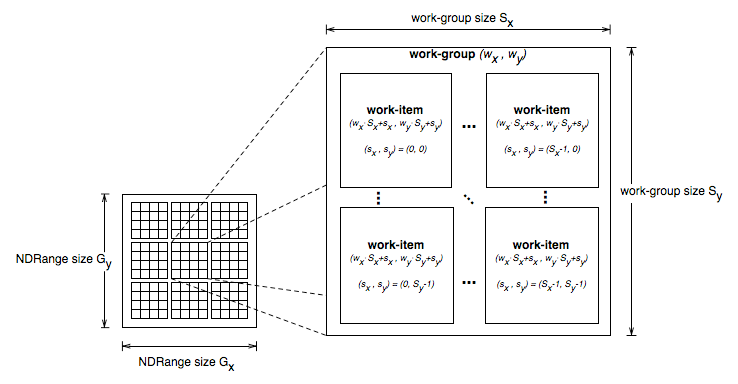
\includegraphics[width=0.8\textwidth]{images/execution-model.png}
  \caption{An example of an NDRange index space showing work-items,
    their global IDs and their mapping onto the pair of work-group and
    local IDs}
  \label{execution-model-figure}
\end{figure}


\subsubsection{Memory model}


``Defines the abstract memory hierarchy that kernels use, regardless of
the actual underlying memory architecture. The memory model closely
resembles current GPU memory hierarchies, although this has not
limited adoptability by other accelerators.''

The memory model specifies 4 distinct memory regions that a work-item
has access to:

\begin{itemize}
\item \textbf{Global Memory}: Similar to the main memory of a desktop
  computer. This memory is visible for all work-items, and is the main
  storage space for kernels input and output data.

\item \textbf{Constant Memory}: This memory is intended for values
  which don't change during execution, and is likely needed by all
  work-items simultaneously during execution. Constant like $\pi$,
  look-up tables of $\sin$ and $\cos$ values, etc. The memory is
  read only, and visible for all work-items.

\item \textbf{Local Memory}: This memory is shared by all work-items
  in the same work-group, with read and write access. It is a
  scratchpad memory, commonly implemented in devices as on-chip memory,
  providing low latency and high bandwidth but at a limited amount.

\item \textbf{Private Memory}: Private memory is unique for each
  work-item, used to store local variables and non-pointer kernel
  arguments.

\end{itemize}

How each of these memory types are implemented is up the vendors. For
GPUs, each of these memory types corresponds to physical memories on
most device. Global memory is mapped to the cards DRAM, constant
memory to a cached region of the DRAM, local memory to the cache on
each multiprocessor, and private memory to the cores registers.

\begin{figure}[h]
  \centering
  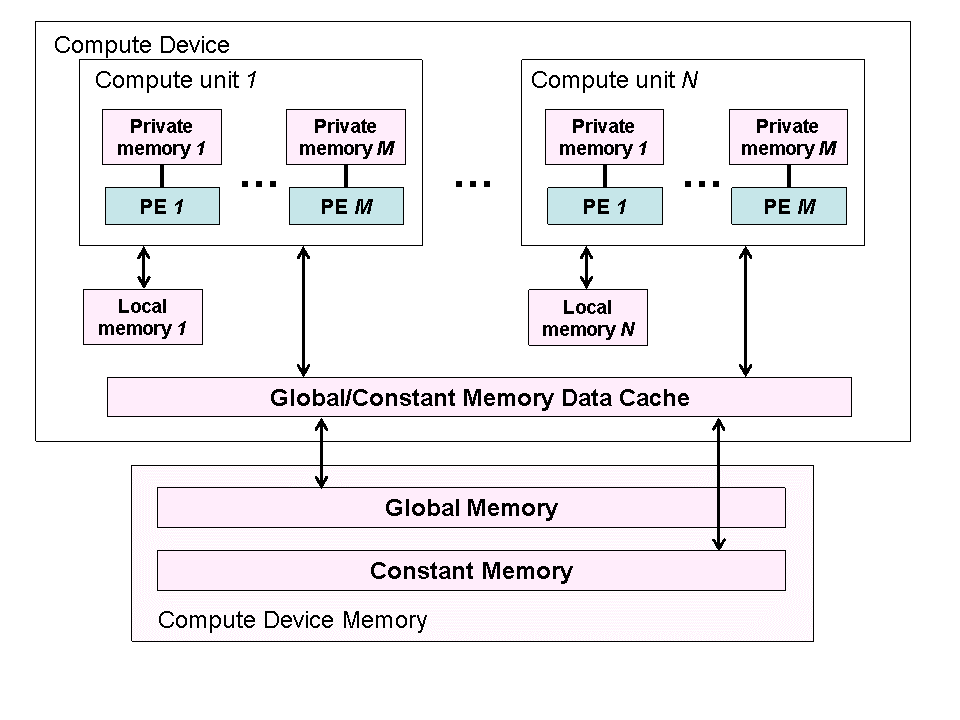
\includegraphics[width=0.8\textwidth]{images/memory-model.png}
  \caption{Conceptual OpenCL device architecture with processing
    elements (PE), compute units and devices. The host is not shown.}
  \label{execution-model-figure}
\end{figure}



\subsubsection{Programming model}

``Defines how the concurrency model is mapped to physical hardware.''

OpenCLs execution model supports both data parallel and task parallel
programming models. The data parallel programming model defines a
computation in terms of a sequence of instruction applied to multiple
elements of a memory object. The NDRange from the execution model
defines how many work-items are used, and how it is mapped to the
data.


\subsection{OpenCL Kernels}

An OpenCL kernel is a kind of function written in OpenCL-C that is
executed by an OpenCL capable device. OpenCL-C is based on C99, with
some restrictions and added extensions. The most noticeable
restrictions include no recursion and no function pointers. The
included extensions are new vector data types like int4, float4 etc,
2D and 3D image types, and some new built-in functions for math,
efficient control-flow, and work-item synchronization and work-item
identifiers.

When writing concurrent programs for a CPU, the programmer needs to
consider the physical resources available (CPU cores) and the overhead
of creating and switching between threads. With OpenCL, the main goal
is to express the problem in a data-parallel way. Often this means
assigning a work-item for each iteration of a loop.

For example; a serial single-CPU function for vector addition might
look something like listing \ref{lst:c-vectoradd}. The function takes
4 arguments; input vector A and B, and the output vector C, all with N
elements. Each iteration in the for-loop adds the corresponding
elements in A and B and stores the result in C.

\begin{lstlisting}[label={lst:c-vectoradd},caption=Serial C vector
    addition function]
  void vectorAdd(int *A, int *B, int *C, int N) {
    for(int i = 0; i < N; i++) 
      C[i] = A[i] + B[i];
  }
\end{lstlisting}

The OpenCL kernel listed in \ref{lst:opencl-vectoradd} achieves the
same output. N instances of this function is generated (as work-items)
and put in the execution queue of the contexts device, which executes
them however the OpenCL runtime deems fit. The devices resources
dictates how many of these kernels can execute in parallel.

\begin{lstlisting}[label={lst:opencl-vectoradd}, caption=OpenCL kernel
    for vector addition]

  __kernel void vectorAdd(__global int *A, 
                          __global int *B, 
                          __global int *C) {
    int tid = get_global_id(0);
    C[tid] = A[tid] + B[tid];
  }
\end{lstlisting}


\section{GPU Optimization Strategies}

There are many considerations that need to be taken into account when
programming for efficiency on a GPU. Although OpenCL programs are
portable, the same application might not be as effective on a CPU as
it is on a GPU. This section will explain some of the optimization
strategies useful for the Nvidia GPU used in this thesis, with a focus
on the ones implemented in chapter \ref{eval-chapter}. More
information is available online from Nvidias Best Practice
article\cite{nvidia-best-practice}.


\begin{itemize}

\item \textbf{Memory optimizations}: a GPUs memory is divided into different
  types, with different properties and sizes, so choosing the best
  memory type for the job is important.

\item \textbf{NDRanges optimizations}: Choosing the best work-group
  sizes to utilize as much of the multiprocessors resources.

\item \textbf{Instruction optimizations}: Some instructions use fewer
  clock cycles than others.

\item \textbf{Control flow}: Execution branching can force the GPU to
  execute parallel code serially, so careful thought and organization
  is important.

\end{itemize}

These strategies applies 

\subsection{Memory Optimizations}

Effectively using the GPUs memory correctly can net large performance
gains. OpenCLs memory model closely resembles current GPUs memory
hierarchy (as shown in \ref{fig:memory-model-figure}), and include
\textit{global}, \textit{local}, \textit{shared}, \textit{texture},
\textit{registers}, \textit{constant} and \textit{texture}. Table
\ref{table:memory-properties} lists the properties of each memory
space.

\begin{table}
  \begin{tabular}{|l|l|l|l|l|l|}
    \hline
    Memory Space & Location on/off chip & Cached & Access & Scope                & Lifetime        \\ \hline
    Register     & on                   & n/a    & r/w    & 1 thread             & thread          \\
    Local        & off                  & no     & r/w    & 1 thread             & thread          \\
    Shared       & on                   & n/a    & r/w    & all threads in block & block           \\
    Global       & off                  & no     & r/w    & all threads and host & host allocation \\
    Constant     & off                  & yes    & r      & all threads and host & host allocation \\
    Texture      & off                  & yes    & r      & all threads and host & host allocation \\
    \hline
  \end{tabular}
  \label{table:memory-properties}
  \caption{List of the Nvidia GeForce 460 GTX memory spaces on the and their properties}
\end{table}

The simplest implementations can use global memory exclusively. But,
accessing global memory on a GPU is by far the slowest operation
available, so reading and writing to it without a care will work, but
impacts the performance. Smart use of all the memory spaces will
increase performance significantly. Constant memory can be used for
look-up tables and constant values, local memory for sharing data
between work-items, texture memory to exploit the cache, and so on. 

\subsubsection{Global Memory Access Patterns}
\label{sect:global-memory-optimization}
One of the most important performance considerations is how this
global memory is accessed. Each store and load operation to the memory
is done by half warps (16 threads), coalesced in as few as one
transaction, in 32-, 64- or 128-byte segments. The exact number of
threads and the segment sizes depends on the GPU and the data type,
and newer GPUs with higher compute capability are more lenient on how
each data segment is laid out, but the general principle is that few
transactions can transfer a lot of data.


\begin{figure}[h]
  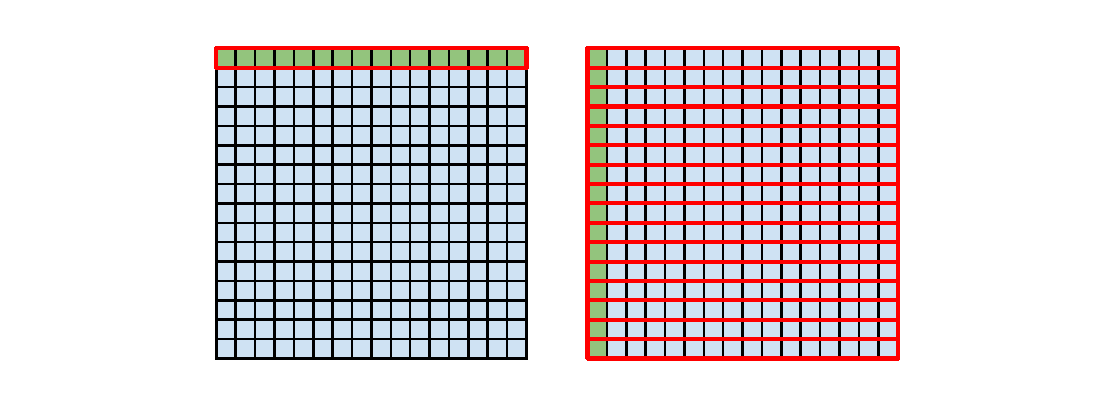
\includegraphics[width=\textwidth]{images/coalesced-access.pdf}
  \caption{Grossly simplified demonstration of how sequential data
    (left group) can be accessed in 1 transaction by a half warp,
    while strided data (right group) results in 16 transactions, where
    only 1 block of data from each read is used.}
  \label{fig:execution-model-figure}
\end{figure}

As seen in figure \ref{fig:execution-model-figure}, laying out the
data needed by the application correctly can increase the bandwidth on
memory transfers greatly.

\begin{lstlisting}[label={lst:coalesced_test}, caption=Copy kernel
  with offset argument]
  __kernel void offsetCopy(__global float *odata,
                           __global float* idata,
                           int offset)
  {
    int xid = get_global_id(0) + offset;
    odata[xid] = idata[xid];
  }
\end{lstlisting}

Misaligned data accesses can be demonstrated with the simple copy
kernel listed in \ref{lst:coalesced_test}. This kernel is launched 32
times with the offset parameter incremented by 1 for each kernel.
Figure \ref{fig:coalesced-performance} shows measurements for 2 Nvidia
devices; GeForce GTX 280 with compute capability 1.3 and GeForce GTX
8800 with compute capability 1.0.

\begin{figure}[h]
  \centering
  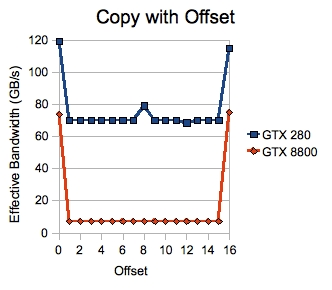
\includegraphics[width=0.5\textwidth]{images/coalesced-performance.png}
  \caption{Performance decrease with misaligned accesses}
  \label{fig:coalesced-performance}
\end{figure}

With offset that are multiples of 16, accesses can be done with 1
transaction per half-warp for the highest bandwidth possible.
Otherwise, 16 transactions per half-warp are issued, resulting in a
performance degradation of at least 8x, because 32 bytes are fetched
per access, but only 4 bytes of those reads are kept.

\subsubsection{Local memory}
\label{sect:local-mem-optimization}

The OpenCL Local memory space is mapped to the GPUs on-chip shared
memory, which provides very low latency and very high throughput
compared to the global memory. The memory is also visible for all
work-items in the same work-group, which lets them share data. This is
especially important for kernels where multiple work-items might need
the same data. A typical strategy for these kernels is to begin with
all threads cooperating in reading a section of data from global
memory into the work-groups local memory, resulting in a single global
read per value needed. 


Local memory is very limited in size, and rigid rules needs to be
follow in order to achieve the maximum performance. The memory is
divided into memory banks of equal size that can be accessed
simultaneously by threads in warps. If multiple threads of a warp need
access to the same memory bank, a bank-conflict happens, and the
request is serialized. However, if all threads of the warp accesses
the same memory bank, there is no bank-conflict. Understanding the
layout of these banks, and laying out data in the correctly can
improve the performance. The exact values and speed of the memory
varies with the compute capability of the GPU, but the principals are
the same for them all.

\subsection{NDRange optimizations}
\label{sect:ndrange-optimization}



\subsection{Instruction optimizations}
\label{sect:instruction-optimization}

\subsection{Control flow}
\label{sect:control-flow}

\section{Depth Estimation on a Parallel Architecture}

This architecture fits the problem of estimating depth perfectly.
Estimating depth is a very data-parallel task, meaning that each pixel
in the resulting depth map can be calculated independent of the other
pixels, in parallel.

An example of a non-data-parallel task is summing up the values in an
array. This is a sequential task, in that each addition of values is
dependent on the previous addition. It is possible to parallelize this
task, but its nature is not data-parallel. For this task, using more
cores to will not increase the performance.

Box filtering is an easy to understand example of a data-parallel
task. The algorithm for the filter is basically; each pixel in the
original image is written into a new image as an average of that
pixels surrounding pixels.

In depth estimation, block matching algorithms have a similar nature
to that of box filtering; each output pixel can be processed
completely on its own. More cores means more tasks can be scheduled in
parallel.

As we'll see in chapter \ref{eval-chapter}, the performance increase
is formidable.
